\documentclass{article}\usepackage[]{graphicx}\usepackage[]{xcolor}
% maxwidth is the original width if it is less than linewidth
% otherwise use linewidth (to make sure the graphics do not exceed the margin)
\makeatletter
\def\maxwidth{ %
  \ifdim\Gin@nat@width>\linewidth
    \linewidth
  \else
    \Gin@nat@width
  \fi
}
\makeatother

\definecolor{fgcolor}{rgb}{0.345, 0.345, 0.345}
\newcommand{\hlnum}[1]{\textcolor[rgb]{0.686,0.059,0.569}{#1}}%
\newcommand{\hlstr}[1]{\textcolor[rgb]{0.192,0.494,0.8}{#1}}%
\newcommand{\hlcom}[1]{\textcolor[rgb]{0.678,0.584,0.686}{\textit{#1}}}%
\newcommand{\hlopt}[1]{\textcolor[rgb]{0,0,0}{#1}}%
\newcommand{\hlstd}[1]{\textcolor[rgb]{0.345,0.345,0.345}{#1}}%
\newcommand{\hlkwa}[1]{\textcolor[rgb]{0.161,0.373,0.58}{\textbf{#1}}}%
\newcommand{\hlkwb}[1]{\textcolor[rgb]{0.69,0.353,0.396}{#1}}%
\newcommand{\hlkwc}[1]{\textcolor[rgb]{0.333,0.667,0.333}{#1}}%
\newcommand{\hlkwd}[1]{\textcolor[rgb]{0.737,0.353,0.396}{\textbf{#1}}}%
\let\hlipl\hlkwb

\usepackage{framed}
\makeatletter
\newenvironment{kframe}{%
 \def\at@end@of@kframe{}%
 \ifinner\ifhmode%
  \def\at@end@of@kframe{\end{minipage}}%
  \begin{minipage}{\columnwidth}%
 \fi\fi%
 \def\FrameCommand##1{\hskip\@totalleftmargin \hskip-\fboxsep
 \colorbox{shadecolor}{##1}\hskip-\fboxsep
     % There is no \\@totalrightmargin, so:
     \hskip-\linewidth \hskip-\@totalleftmargin \hskip\columnwidth}%
 \MakeFramed {\advance\hsize-\width
   \@totalleftmargin\z@ \linewidth\hsize
   \@setminipage}}%
 {\par\unskip\endMakeFramed%
 \at@end@of@kframe}
\makeatother

\definecolor{shadecolor}{rgb}{.97, .97, .97}
\definecolor{messagecolor}{rgb}{0, 0, 0}
\definecolor{warningcolor}{rgb}{1, 0, 1}
\definecolor{errorcolor}{rgb}{1, 0, 0}
\newenvironment{knitrout}{}{} % an empty environment to be redefined in TeX

\usepackage{alltt}
\usepackage[sc]{mathpazo}
\renewcommand{\sfdefault}{lmss}
\renewcommand{\ttdefault}{lmtt}
\usepackage[T1]{fontenc}
\usepackage{geometry}
\geometry{verbose,tmargin=2.5cm,bmargin=2.5cm,lmargin=2.5cm,rmargin=2.5cm}
\setcounter{secnumdepth}{2}
\setcounter{tocdepth}{2}
\usepackage[unicode=true,pdfusetitle,
 bookmarks=true,bookmarksnumbered=true,bookmarksopen=true,bookmarksopenlevel=2,
 breaklinks=false,pdfborder={0 0 1},backref=false,colorlinks=false]
 {hyperref}
\hypersetup{
 pdfstartview={XYZ null null 1}}

\makeatletter
%%%%%%%%%%%%%%%%%%%%%%%%%%%%%% User specified LaTeX commands.
\renewcommand{\textfraction}{0.05}
\renewcommand{\topfraction}{0.8}
\renewcommand{\bottomfraction}{0.8}
\renewcommand{\floatpagefraction}{0.75}

\makeatother
\IfFileExists{upquote.sty}{\usepackage{upquote}}{}
\begin{document}








The results below are generated from an R script.

\begin{knitrout}
\definecolor{shadecolor}{rgb}{0.969, 0.969, 0.969}\color{fgcolor}\begin{kframe}
\begin{alltt}
\hlkwd{library}\hlstd{(}\hlstr{"tidyverse"}\hlstd{)}
\end{alltt}


{\ttfamily\noindent\itshape\color{messagecolor}{\#\# -- Attaching packages ------------------------------------------------- tidyverse 1.3.2 --\\\#\# v ggplot2 3.4.0 \ \ \ \ \ v purrr \ \ 0.3.5 \\\#\# v tibble \ 3.1.8 \ \ \ \ \ v dplyr \ \ 1.0.10\\\#\# v tidyr \ \ 1.2.1 \ \ \ \ \ v stringr 1.4.1 \\\#\# v readr \ \ 2.1.3 \ \ \ \ \ v forcats 0.5.2 \\\#\# -- Conflicts ---------------------------------------------------- tidyverse\_conflicts() --\\\#\# x readr::edition\_get() \ \ masks testthat::edition\_get()\\\#\# x dplyr::filter() \ \ \ \ \ \ \ masks stats::filter()\\\#\# x purrr::is\_null() \ \ \ \ \ \ masks testthat::is\_null()\\\#\# x dplyr::lag() \ \ \ \ \ \ \ \ \ \ masks stats::lag()\\\#\# x readr::local\_edition() masks testthat::local\_edition()\\\#\# x dplyr::matches() \ \ \ \ \ \ masks tidyr::matches(), testthat::matches()}}\begin{alltt}
\hlkwd{library}\hlstd{(}\hlstr{"gridExtra"}\hlstd{)}
\end{alltt}


{\ttfamily\noindent\itshape\color{messagecolor}{\#\# \\\#\# Attaching package: 'gridExtra'\\\#\# \\\#\# The following object is masked from 'package:dplyr':\\\#\# \\\#\# \ \ \ \ combine}}\begin{alltt}
\hlkwd{library}\hlstd{(}\hlstr{"ggthemes"}\hlstd{)}
\hlkwd{library}\hlstd{(}\hlstr{"png"}\hlstd{)}
\hlkwd{library}\hlstd{(}\hlstr{"scales"}\hlstd{)}
\end{alltt}


{\ttfamily\noindent\itshape\color{messagecolor}{\#\# \\\#\# Attaching package: 'scales'\\\#\# \\\#\# The following object is masked from 'package:purrr':\\\#\# \\\#\# \ \ \ \ discard\\\#\# \\\#\# The following object is masked from 'package:readr':\\\#\# \\\#\# \ \ \ \ col\_factor}}\begin{alltt}
\hlkwd{library}\hlstd{(}\hlstr{"simputation"}\hlstd{)}
\hlkwd{library}\hlstd{(}\hlstr{"naniar"}\hlstd{)}
\end{alltt}


{\ttfamily\noindent\itshape\color{messagecolor}{\#\# \\\#\# Attaching package: 'naniar'\\\#\# \\\#\# The following object is masked from 'package:simputation':\\\#\# \\\#\# \ \ \ \ impute\_median}}\begin{alltt}
\hlkwd{library}\hlstd{(}\hlstr{"lubridate"}\hlstd{)}
\end{alltt}


{\ttfamily\noindent\itshape\color{messagecolor}{\#\# Loading required package: timechange\\\#\# \\\#\# Attaching package: 'lubridate'\\\#\# \\\#\# The following objects are masked from 'package:base':\\\#\# \\\#\# \ \ \ \ date, intersect, setdiff, union}}\begin{alltt}
\hlkwd{library}\hlstd{(}\hlstr{"magick"}\hlstd{)}
\end{alltt}


{\ttfamily\noindent\itshape\color{messagecolor}{\#\# Linking to ImageMagick 6.9.12.3\\\#\# Enabled features: cairo, fontconfig, freetype, heic, lcms, pango, raw, rsvg, webp\\\#\# Disabled features: fftw, ghostscript, x11}}\begin{alltt}
\hlkwd{library}\hlstd{(}\hlstr{"rpart"}\hlstd{)}
\hlkwd{library}\hlstd{(}\hlstr{"visdat"}\hlstd{)}
\hlkwd{library}\hlstd{(}\hlstr{"patchwork"}\hlstd{)}
\hlkwd{library}\hlstd{(}\hlstr{"withr"}\hlstd{)}
\hlkwd{library}\hlstd{(}\hlstr{"targets"}\hlstd{)}
\end{alltt}


{\ttfamily\noindent\itshape\color{messagecolor}{\#\# \\\#\# Attaching package: 'targets'\\\#\# \\\#\# The following object is masked from 'package:testthat':\\\#\# \\\#\# \ \ \ \ matches}}\begin{alltt}
\hlkwd{library}\hlstd{(}\hlstr{"tidyverse"}\hlstd{)}
\hlkwd{library}\hlstd{(}\hlstr{"janitor"}\hlstd{)}
\end{alltt}


{\ttfamily\noindent\itshape\color{messagecolor}{\#\# \\\#\# Attaching package: 'janitor'\\\#\# \\\#\# The following objects are masked from 'package:stats':\\\#\# \\\#\# \ \ \ \ chisq.test, fisher.test}}\begin{alltt}
\hlkwd{library}\hlstd{(}\hlstr{"knitr"}\hlstd{)}
\hlkwd{library}\hlstd{(}\hlstr{"cowplot"}\hlstd{)}
\end{alltt}


{\ttfamily\noindent\itshape\color{messagecolor}{\#\# \\\#\# Attaching package: 'cowplot'\\\#\# \\\#\# The following object is masked from 'package:patchwork':\\\#\# \\\#\# \ \ \ \ align\_plots\\\#\# \\\#\# The following object is masked from 'package:lubridate':\\\#\# \\\#\# \ \ \ \ stamp\\\#\# \\\#\# The following object is masked from 'package:ggthemes':\\\#\# \\\#\# \ \ \ \ theme\_map}}\end{kframe}
\end{knitrout}
\begin{knitrout}
\definecolor{shadecolor}{rgb}{0.969, 0.969, 0.969}\color{fgcolor}\begin{kframe}
\begin{alltt}
\hlstd{housing_raw} \hlkwb{<-}
  \hlkwd{read_csv}\hlstd{(}\hlstr{"data/melbourne_housing_raw.csv"}\hlstd{)} \hlopt
  \hlkwd{clean_names}\hlstd{()} \hlopt
  \hlkwd{rename}\hlstd{(}\hlkwc{region_name} \hlstd{= regionname,}
         \hlkwc{property_count} \hlstd{= propertycount)} \hlopt
  \hlkwd{mutate}\hlstd{(}\hlkwc{date} \hlstd{=} \hlkwd{dmy}\hlstd{(date))} \hlopt
  \hlkwd{rename}\hlstd{(}\hlkwc{latitude} \hlstd{= lattitude,}
         \hlkwc{longitude} \hlstd{= longtitude)} \hlopt
  \hlcom{# let's create monthly quarters}
  \hlkwd{mutate}\hlstd{(}\hlkwc{yr_qtr} \hlstd{=} \hlkwd{as.ordered}\hlstd{(}\hlkwd{quarter}\hlstd{(date,}
                                     \hlkwc{with_year} \hlstd{=} \hlnum{TRUE}\hlstd{,}
                                     \hlkwc{fiscal_start} \hlstd{=} \hlnum{1}\hlstd{)))} \hlopt
  \hlcom{# drop price}
  \hlkwd{drop_na}\hlstd{(price)} \hlopt
  \hlcom{# make price the log of price}
  \hlkwd{mutate}\hlstd{(}\hlkwc{price} \hlstd{=} \hlkwd{log10}\hlstd{(price))}
\end{alltt}


{\ttfamily\noindent\color{warningcolor}{\#\# Warning: One or more parsing issues, call `problems()` on your data frame for details, e.g.:\\\#\# \ \ dat <- vroom(...)\\\#\# \ \ problems(dat)}}

{\ttfamily\noindent\itshape\color{messagecolor}{\#\# Rows: 34857 Columns: 20\\\#\# -- Column specification ------------------------------------------------------------------\\\#\# Delimiter: "{},"{}\\\#\# chr \ (7): Suburb, Type, Method, SellerG, Date, CouncilArea, Regionname\\\#\# dbl (13): Rooms, Price, Distance, Postcode, Bedroom2, Bathroom, Car, Landsize, Buildin...\\\#\# \\\#\# i Use `spec()` to retrieve the full column specification for this data.\\\#\# i Specify the column types or set `show\_col\_types = FALSE` to quiet this message.}}\begin{alltt}
\hlcom{# compact down the seller levels}
\hlstd{count_dat} \hlkwb{<-} \hlkwd{count}\hlstd{(housing_raw,seller_g)} \hlopt
  \hlkwd{arrange}\hlstd{(}\hlopt{-}\hlstd{n)} \hlopt
  \hlkwd{mutate}\hlstd{(}\hlkwc{cumu} \hlstd{=} \hlkwd{cumsum}\hlstd{(n),}
         \hlkwc{pct} \hlstd{= cumu} \hlopt{/} \hlkwd{nrow}\hlstd{(housing_raw),}
         \hlkwc{pct_change} \hlstd{= pct} \hlopt{-} \hlkwd{lag}\hlstd{(pct))} \hlopt
  \hlkwd{rowid_to_column}\hlstd{()} \hlopt
  \hlkwd{mutate}\hlstd{(}\hlkwc{seller} \hlstd{=} \hlkwd{case_when}\hlstd{(}
    \hlstd{pct} \hlopt{<} \hlnum{0.52} \hlopt{~} \hlkwd{as.character}\hlstd{(seller_g),}
    \hlstd{pct} \hlopt{>} \hlnum{0.52} \hlopt{&} \hlstd{pct} \hlopt{<} \hlnum{0.60} \hlopt{~} \hlstr{"seller_g1"}\hlstd{,}
    \hlstd{pct} \hlopt{>} \hlnum{0.60} \hlopt{&} \hlstd{pct} \hlopt{<} \hlnum{0.65} \hlopt{~} \hlstr{"seller_g2"}\hlstd{,}
    \hlstd{pct} \hlopt{>} \hlnum{0.65} \hlopt{&} \hlstd{pct} \hlopt{<} \hlnum{0.70} \hlopt{~} \hlstr{"seller_g3"}\hlstd{,}
    \hlstd{pct} \hlopt{>} \hlnum{0.70} \hlopt{&} \hlstd{pct} \hlopt{<} \hlnum{0.75} \hlopt{~} \hlstr{"seller_g4"}\hlstd{,}
    \hlstd{pct} \hlopt{>} \hlnum{0.75} \hlopt{&} \hlstd{pct} \hlopt{<} \hlnum{0.80} \hlopt{~} \hlstr{"seller_g5"}\hlstd{,}
    \hlstd{pct} \hlopt{>} \hlnum{0.80} \hlopt{&} \hlstd{pct} \hlopt{<} \hlnum{0.85} \hlopt{~} \hlstr{"seller_g6"}\hlstd{,}
    \hlstd{pct} \hlopt{>} \hlnum{0.85} \hlopt{&} \hlstd{pct} \hlopt{<} \hlnum{0.90} \hlopt{~} \hlstr{"seller_g6"}\hlstd{,}
    \hlstd{pct} \hlopt{>} \hlnum{0.90} \hlopt{&} \hlstd{pct} \hlopt{<} \hlnum{0.95} \hlopt{~} \hlstr{"seller_g6"}\hlstd{,}
    \hlstd{pct} \hlopt{>} \hlnum{0.95} \hlopt{~} \hlstr{"seller_g5"}
  \hlstd{))}

\hlcom{# drop these three variables, as we won't use them in analysis, they}
\hlcom{# would need extensive recoding}

\hlstd{housing} \hlkwb{<-} \hlstd{housing_raw} \hlopt
  \hlkwd{mutate_if}\hlstd{(is.character, as.factor)} \hlopt
  \hlkwd{mutate_at}\hlstd{(}\hlkwd{vars}\hlstd{(rooms,}
                 \hlstd{bedroom2,}
                 \hlstd{bathroom,}
                 \hlstd{car),}
            \hlstd{as.factor)} \hlopt
  \hlcom{# recode / collapse factors with many levels and few obs}
  \hlkwd{mutate}\hlstd{(}\hlkwc{bathroom} \hlstd{=} \hlkwd{fct_other}\hlstd{(bathroom,}
                              \hlkwc{drop} \hlstd{=} \hlkwd{c}\hlstd{(}\hlstr{"4"}\hlstd{,} \hlstr{"5"}\hlstd{,} \hlstr{"6"}\hlstd{,} \hlstr{"7"}\hlstd{,} \hlstr{"8"}\hlstd{,} \hlstr{"9"}\hlstd{),}
                              \hlkwc{other_level} \hlstd{=} \hlstr{"4+"}\hlstd{))} \hlopt
  \hlkwd{mutate}\hlstd{(}\hlkwc{bedroom2} \hlstd{=} \hlkwd{fct_other}\hlstd{(bedroom2,}
                              \hlkwc{drop} \hlstd{=} \hlkwd{c}\hlstd{(}\hlstr{"5"}\hlstd{,} \hlstr{"6"}\hlstd{,} \hlstr{"7"}\hlstd{,} \hlstr{"8"}\hlstd{,} \hlstr{"9"}\hlstd{,} \hlstr{"10"}\hlstd{,}
                                       \hlstr{"12"}\hlstd{,} \hlstr{"16"}\hlstd{,} \hlstr{"20"}\hlstd{),}
                              \hlkwc{other_level} \hlstd{=} \hlstr{"5+"}\hlstd{))} \hlopt
  \hlkwd{mutate}\hlstd{(}\hlkwc{rooms} \hlstd{=} \hlkwd{fct_other}\hlstd{(rooms,}
                           \hlkwc{drop} \hlstd{=} \hlkwd{c}\hlstd{(}\hlstr{"6"}\hlstd{,} \hlstr{"7"}\hlstd{,} \hlstr{"8"}\hlstd{,} \hlstr{"9"}\hlstd{,} \hlstr{"10"}\hlstd{,}
                                    \hlstr{"12"}\hlstd{,} \hlstr{"16"}\hlstd{),}
                           \hlkwc{other_level} \hlstd{=} \hlstr{"6+"}\hlstd{))} \hlopt
  \hlkwd{mutate}\hlstd{(}\hlkwc{car} \hlstd{=} \hlkwd{fct_other}\hlstd{(car,}
                         \hlkwc{drop} \hlstd{=} \hlkwd{c}\hlstd{(}\hlstr{"4"}\hlstd{,} \hlstr{"5"}\hlstd{,} \hlstr{"6"}\hlstd{,} \hlstr{"7"}\hlstd{,} \hlstr{"8"}\hlstd{,} \hlstr{"9"}\hlstd{,} \hlstr{"10"}\hlstd{,}
                                  \hlstr{"11"}\hlstd{,} \hlstr{"18"}\hlstd{),}
                         \hlkwc{other_level} \hlstd{=} \hlstr{"4+"}\hlstd{))} \hlopt
  \hlkwd{left_join}\hlstd{(}\hlkwd{select}\hlstd{(count_dat, seller_g, seller),} \hlkwc{by} \hlstd{=} \hlstr{"seller_g"}\hlstd{)}  \hlopt
  \hlcom{# drop seller_g}
  \hlkwd{select}\hlstd{(}\hlopt{-}\hlstd{seller_g)} \hlopt
  \hlkwd{mutate}\hlstd{(}\hlkwc{seller} \hlstd{=} \hlkwd{as.factor}\hlstd{(seller))}
\end{alltt}
\end{kframe}
\end{knitrout}
\begin{knitrout}
\definecolor{shadecolor}{rgb}{0.969, 0.969, 0.969}\color{fgcolor}\begin{kframe}
\begin{alltt}
\hlstd{p1} \hlkwb{<-} \hlkwd{ggplot}\hlstd{(oceanbuoys,}
       \hlkwd{aes}\hlstd{(}\hlkwc{x} \hlstd{= humidity,}
           \hlkwc{y} \hlstd{= air_temp_c))} \hlopt{+}
  \hlkwd{geom_point}\hlstd{(}\hlkwc{size} \hlstd{=} \hlnum{0.5}\hlstd{)} \hlopt{+}
  \hlkwd{theme}\hlstd{(}\hlkwc{aspect.ratio} \hlstd{=} \hlnum{1}\hlstd{)} \hlopt{+}
  \hlkwd{labs}\hlstd{(}\hlkwc{x} \hlstd{=} \hlstr{"Humidity"}\hlstd{,}
       \hlkwc{y} \hlstd{=} \hlstr{"Air Temperature (C)"}\hlstd{)}

\hlstd{p1} \hlopt{+} \hlstd{grid}\hlopt{::}\hlkwd{textGrob}\hlstd{(}
  \hlkwc{label} \hlstd{=} \hlstr{"Warning message:
removed 171 rows containing 
missing values (geom_point)."}\hlstd{,}
\hlkwc{gp} \hlstd{= grid}\hlopt{::}\hlkwd{gpar}\hlstd{(}\hlkwc{fontsize} \hlstd{=} \hlnum{14}\hlstd{,}
                \hlkwc{fontfamily} \hlstd{=} \hlstr{"Courier"}\hlstd{,}
                \hlkwc{col} \hlstd{=} \hlstr{"salmon"}\hlstd{,}
                \hlkwc{fontface} \hlstd{=} \hlstr{"bold"}\hlstd{))}
\end{alltt}
\end{kframe}\begin{figure}

{\centering \includegraphics[width=0.75\linewidth]{figure/code-Rnwwarning-1} 

}

\caption[How \pkg{ggplot2} behaves when displaying missing values]{How \pkg{ggplot2} behaves when displaying missing values. A warning message is displayed, but missing values are not shown in the plot.}\label{fig:warning}
\end{figure}

\end{knitrout}

\begin{knitrout}
\definecolor{shadecolor}{rgb}{0.969, 0.969, 0.969}\color{fgcolor}\begin{kframe}
\begin{alltt}
\hlstd{gg_boxplot} \hlkwb{<-}  \hlkwa{function}\hlstd{(}\hlkwc{data}\hlstd{)\{}
  \hlkwd{ggplot}\hlstd{(data,}
       \hlkwd{aes_string}\hlstd{(}\hlkwc{x} \hlstd{=} \hlstr{"year"}\hlstd{,}
                  \hlkwc{y} \hlstd{=} \hlstr{"score"}\hlstd{))} \hlopt{+}
  \hlkwd{geom_boxplot}\hlstd{()}
\hlstd{\}}

\hlstd{p1} \hlkwb{<-} \hlkwd{gg_boxplot}\hlstd{(school_scores_all} \hlopt \hlkwd{filter}\hlstd{(NA_type} \hlopt{==} \hlstr{"complete"}\hlstd{))}
\end{alltt}


{\ttfamily\noindent\color{warningcolor}{\#\# Warning: `aes\_string()` was deprecated in ggplot2 3.0.0.\\\#\# i Please use tidy evaluation ideoms with `aes()`}}\begin{alltt}
\hlstd{p2} \hlkwb{<-} \hlkwd{gg_boxplot}\hlstd{(school_scores_all} \hlopt \hlkwd{filter}\hlstd{(NA_type} \hlopt{==} \hlstr{"year_NA"}\hlstd{))}
\hlstd{p3} \hlkwb{<-} \hlkwd{gg_boxplot}\hlstd{(school_scores_all} \hlopt \hlkwd{filter}\hlstd{(NA_type} \hlopt{==} \hlstr{"score_NA"}\hlstd{))}
\hlstd{p4} \hlkwb{<-} \hlkwd{gg_boxplot}\hlstd{(school_scores_all} \hlopt \hlkwd{filter}\hlstd{(NA_type} \hlopt{==} \hlstr{"both_NA"}\hlstd{))}

\hlkwd{plot_grid}\hlstd{(p1, p2, p3, p4,} \hlkwc{nrow} \hlstd{=} \hlnum{1}\hlstd{,} \hlkwc{labels} \hlstd{= LETTERS[}\hlnum{1}\hlopt{:}\hlnum{4}\hlstd{])}
\end{alltt}


{\ttfamily\noindent\color{warningcolor}{\#\# Warning: Removed 11 rows containing non-finite values (`stat\_boxplot()`).}}

{\ttfamily\noindent\color{warningcolor}{\#\# Warning: Removed 13 rows containing non-finite values (`stat\_boxplot()`).}}\end{kframe}\begin{figure}

{\centering \includegraphics[width=1\linewidth]{figure/code-Rnwgg-box-na-1} 

}

\caption[\pkg{ggplot2} provides different visualizations depending on what type of data has missing values for data of student test scores in school year]{\pkg{ggplot2} provides different visualizations depending on what type of data has missing values for data of student test scores in school year. (A) Data is complete; (B) Missings are only in year - an additional "NA" boxplot is created; (C) Missings only in scores, no additional missingness information is shown; (D) Missings in both scores and year, additional missing information is shown. The missingness category is only shown when there are missings in categorical variables such as year (plots (B) and (D)). In (C), no missingness information is given on the graphic, despite there being missings in score, and a warning message is displayed about the number of missing values omitted.}\label{fig:gg-box-na}
\end{figure}

\end{knitrout}
\begin{knitrout}
\definecolor{shadecolor}{rgb}{0.969, 0.969, 0.969}\color{fgcolor}\begin{kframe}
\begin{alltt}
\hlstd{dat_ms} \hlkwb{<-} \hlkwd{tribble}\hlstd{(}\hlopt{~}\hlstd{x,}    \hlopt{~}\hlstd{y,}     \hlopt{~}\hlstd{z,}
                   \hlnum{1}\hlstd{,}   \hlstr{"A"}\hlstd{,}   \hlopt{-}\hlnum{100}\hlstd{,}
                   \hlnum{3}\hlstd{,} \hlstr{"N/A"}\hlstd{,}    \hlopt{-}\hlnum{99}\hlstd{,}
                  \hlnum{NA}\hlstd{,}   \hlnum{NA}\hlstd{,}     \hlopt{-}\hlnum{98}\hlstd{,}
                 \hlopt{-}\hlnum{99}\hlstd{,}  \hlstr{"E"}\hlstd{,}    \hlopt{-}\hlnum{101}\hlstd{,}
                 \hlopt{-}\hlnum{98}\hlstd{,}  \hlstr{"F"}\hlstd{,}      \hlopt{-}\hlnum{1}\hlstd{)}
\end{alltt}
\end{kframe}
\end{knitrout}
\begin{knitrout}
\definecolor{shadecolor}{rgb}{0.969, 0.969, 0.969}\color{fgcolor}\begin{kframe}
\begin{alltt}
\hlkwd{tibble}\hlstd{(}
  \hlkwc{`Function`} \hlstd{=} \hlkwd{c}\hlstd{(}
    \hlstr{"add_n_miss(data)"}\hlstd{,}
    \hlstr{"add_any_miss(data)"}\hlstd{,}
    \hlstr{"add_prop_miss(data)"}\hlstd{,}
    \hlstr{"add_miss_cluster(data)"}
    \hlstd{),}
  \hlkwc{`Adds column which:`} \hlstd{=} \hlkwd{c}\hlstd{(}
    \hlstr{"contains the number missing values in a row"}\hlstd{,}
    \hlstr{"contains whether there are any missing values in a row"}\hlstd{,}
    \hlstr{"contains the proportion of missing values in a row"}\hlstd{,}
    \hlstr{"contains the missing value cluster"}
  \hlstd{))} \hlopt
    \hlkwd{kable}\hlstd{(}\hlkwc{caption} \hlstd{=} \hlstr{'Overview of the "add" functions in naniar'}\hlstd{)}
\end{alltt}
\end{kframe}\begin{table}

\caption{\label{tab:add-missing-info}Overview of the "add" functions in naniar}
\centering
\begin{tabular}[t]{l|l}
\hline
Function & Adds column which:\\
\hline
add\_n\_miss(data) & contains the number missing values in a row\\
\hline
add\_any\_miss(data) & contains whether there are any missing values in a row\\
\hline
add\_prop\_miss(data) & contains the proportion of missing values in a row\\
\hline
add\_miss\_cluster(data) & contains the missing value cluster\\
\hline
\end{tabular}
\end{table}

\end{knitrout}
\begin{knitrout}
\definecolor{shadecolor}{rgb}{0.969, 0.969, 0.969}\color{fgcolor}\begin{kframe}
\begin{alltt}
\hlkwd{nabular}\hlstd{(dat_ms)}
\end{alltt}
\begin{verbatim}
## # A tibble: 5 x 6
##       x y         z x_NA  y_NA  z_NA 
##   <dbl> <chr> <dbl> <fct> <fct> <fct>
## 1     1 A      -100 !NA   !NA   !NA  
## 2     3 N/A     -99 !NA   !NA   !NA  
## 3    NA <NA>    -98 NA    NA    !NA  
## 4   -99 E      -101 !NA   !NA   !NA  
## 5   -98 F        -1 !NA   !NA   !NA
\end{verbatim}
\end{kframe}
\end{knitrout}
\begin{knitrout}
\definecolor{shadecolor}{rgb}{0.969, 0.969, 0.969}\color{fgcolor}\begin{kframe}
\begin{alltt}
\hlkwd{nabular}\hlstd{(dat_ms)} \hlopt
  \hlkwd{recode_shadow}\hlstd{(}\hlkwc{x} \hlstd{=} \hlkwd{.where}\hlstd{(x} \hlopt{== -}\hlnum{99} \hlopt{~} \hlstr{"broken_sensor"}\hlstd{))}
\end{alltt}
\begin{verbatim}
## # A tibble: 5 x 6
##       x y         z x_NA             y_NA  z_NA 
##   <dbl> <chr> <dbl> <fct>            <fct> <fct>
## 1     1 A      -100 !NA              !NA   !NA  
## 2     3 N/A     -99 !NA              !NA   !NA  
## 3    NA <NA>    -98 NA               NA    !NA  
## 4   -99 E      -101 NA_broken_sensor !NA   !NA  
## 5   -98 F        -1 !NA              !NA   !NA
\end{verbatim}
\end{kframe}
\end{knitrout}
\begin{knitrout}
\definecolor{shadecolor}{rgb}{0.969, 0.969, 0.969}\color{fgcolor}\begin{kframe}
\begin{alltt}
\hlstd{aq_imputed} \hlkwb{<-} \hlkwd{nabular}\hlstd{(airquality)} \hlopt
  \hlkwd{as.data.frame}\hlstd{()} \hlopt
  \hlstd{simputation}\hlopt{::}\hlkwd{impute_lm}\hlstd{(Ozone} \hlopt{~} \hlstd{Temp} \hlopt{+} \hlstd{Wind)} \hlopt
  \hlstd{simputation}\hlopt{::}\hlkwd{impute_lm}\hlstd{(Solar.R} \hlopt{~} \hlstd{Temp} \hlopt{+} \hlstd{Wind)} \hlopt
  \hlkwd{add_label_shadow}\hlstd{()}

\hlkwd{head}\hlstd{(aq_imputed)}
\end{alltt}
\begin{verbatim}
##       Ozone  Solar.R Wind Temp Month Day Ozone_NA Solar.R_NA Wind_NA Temp_NA Month_NA
## 1  41.00000 190.0000  7.4   67     5   1      !NA        !NA     !NA     !NA      !NA
## 2  36.00000 118.0000  8.0   72     5   2      !NA        !NA     !NA     !NA      !NA
## 3  12.00000 149.0000 12.6   74     5   3      !NA        !NA     !NA     !NA      !NA
## 4  18.00000 313.0000 11.5   62     5   4      !NA        !NA     !NA     !NA      !NA
## 5 -11.67673 127.4317 14.3   56     5   5       NA         NA     !NA     !NA      !NA
## 6  28.00000 159.5042 14.9   66     5   6      !NA         NA     !NA     !NA      !NA
##   Day_NA any_missing
## 1    !NA Not Missing
## 2    !NA Not Missing
## 3    !NA Not Missing
## 4    !NA Not Missing
## 5    !NA     Missing
## 6    !NA     Missing
\end{verbatim}
\end{kframe}
\end{knitrout}
\begin{knitrout}
\definecolor{shadecolor}{rgb}{0.969, 0.969, 0.969}\color{fgcolor}\begin{figure}

{\centering \includegraphics[width=1\linewidth]{figure/code-Rnwtrack-impute-example-1} 

}

\caption[Scatterplot (A) and density plots (B and C) of ozone and solar radiation from the airquality dataset containing imputed values from a linear model]{Scatterplot (A) and density plots (B and C) of ozone and solar radiation from the airquality dataset containing imputed values from a linear model. Imputed values are colored green, and data values orange. Imputed values are similar, but slightly trended to the mean.}\label{fig:track-impute-example}
\end{figure}

\end{knitrout}
\begin{knitrout}
\definecolor{shadecolor}{rgb}{0.969, 0.969, 0.969}\color{fgcolor}\begin{table}

\caption{\label{tab:impute-summary-out}Output of \pkg{dplyr} summary statistics of imputed vs non imputed values for the variable "Ozone". The "any\_missing" column denotes imputed values ("Missing", since they were previously missing), and non-imputed values ("Not Missing"). The mean and median values are similar, but the minimum and maximum values are very different.}
\centering
\begin{tabular}[t]{l|r|r|r|r}
\hline
any\_missing & min & mean & median & max\\
\hline
Missing & -16.86418 & 41.22494 & 45.4734 & 78\\
\hline
Not Missing & 1.00000 & 42.09910 & 31.0000 & 168\\
\hline
\end{tabular}
\end{table}

\end{knitrout}
\begin{knitrout}
\definecolor{shadecolor}{rgb}{0.969, 0.969, 0.969}\color{fgcolor}\begin{kframe}


{\ttfamily\noindent\color{warningcolor}{\#\# Warning: `gather\_()` was deprecated in tidyr 1.2.0.\\\#\# i Please use `gather()` instead.\\\#\# i The deprecated feature was likely used in the visdat package.\\\#\# \ \ Please report the issue at <]8;;https://github.com/ropensci/visdat/issueshttps://github.com/ropensci/visdat/issues]8;;>.}}

{\ttfamily\noindent\color{warningcolor}{\#\# Warning: The `guide` argument in `scale\_*()` cannot be `FALSE`. This was deprecated in ggplot2\\\#\# 3.3.4.\\\#\# i Please use "{}none"{} instead.\\\#\# i The deprecated feature was likely used in the naniar package.\\\#\# \ \ Please report the issue at <]8;;https://github.com/njtierney/naniar/issueshttps://github.com/njtierney/naniar/issues]8;;>.}}\end{kframe}\begin{figure}

{\centering \includegraphics[width=0.9\linewidth]{figure/code-Rnwgg-miss-case-var-1} 

}

\caption[Graphical summaries of missingness in the airquality data]{Graphical summaries of missingness in the airquality data. Missings in variables (A) and cases (B), and for an overview of all missingness as a heatmap in (C), and with clustering applied (D). There are missing values in Ozone and Solar.R, with Ozone having more missings. Not many cases have two missings. Most missingness is from cases with one missing value. The default output (C) and ordered by clustering on rows and columns (D). These overviews are made possible using the shadow matrix in long form. There are only missings in ozone and solar radiation, and there appears to be some structure to their missingness.}\label{fig:gg-miss-case-var}
\end{figure}

\end{knitrout}
\begin{knitrout}
\definecolor{shadecolor}{rgb}{0.969, 0.969, 0.969}\color{fgcolor}\begin{kframe}
\begin{alltt}
\hlkwd{gg_miss_upset}\hlstd{(airquality)}
\end{alltt}
\end{kframe}\begin{figure}

{\centering \includegraphics[width=.6\linewidth]{figure/code-Rnwairquality-upset-1} 

}

\caption[The pattern of missingness in the airquality dataset shown in an upset plot]{The pattern of missingness in the airquality dataset shown in an upset plot. Only Ozone and Solar.R have missing values, and Ozone has the most missing values. There are 2 cases where both Solar.R and Ozone have missing values.}\label{fig:airquality-upset}
\end{figure}

\end{knitrout}
\begin{knitrout}
\definecolor{shadecolor}{rgb}{0.969, 0.969, 0.969}\color{fgcolor}\begin{kframe}
\begin{alltt}
\hlstd{airquality} \hlopt
  \hlkwd{nabular}\hlstd{()} \hlopt
  \hlkwd{impute_below_all}\hlstd{()} \hlopt
  \hlkwd{ggplot}\hlstd{(}\hlkwd{aes}\hlstd{(}\hlkwc{x} \hlstd{= Ozone,}
             \hlkwc{fill} \hlstd{= Ozone_NA))} \hlopt{+}
  \hlkwd{geom_histogram}\hlstd{()} \hlopt{+}
  \hlkwd{scale_fill_brewer}\hlstd{(}\hlkwc{palette} \hlstd{=} \hlstr{"Dark2"}\hlstd{)} \hlopt{+}
  \hlkwd{labs}\hlstd{(}\hlkwc{tag} \hlstd{=} \hlstr{"A"}\hlstd{)} \hlopt{+}
  \hlkwd{theme}\hlstd{(}\hlkwc{legend.position} \hlstd{=} \hlstr{"bottom"}\hlstd{)}

\hlstd{airquality} \hlopt
  \hlkwd{nabular}\hlstd{()} \hlopt
\hlkwd{ggplot}\hlstd{(}\hlkwd{aes}\hlstd{(}\hlkwc{x} \hlstd{= Temp))} \hlopt{+}
  \hlkwd{geom_histogram}\hlstd{(}\hlkwc{na.rm} \hlstd{=} \hlnum{TRUE}\hlstd{)} \hlopt{+}
  \hlkwd{facet_wrap}\hlstd{(}\hlopt{~}\hlstd{Ozone_NA)} \hlopt{+}
  \hlkwd{labs}\hlstd{(}\hlkwc{tag} \hlstd{=} \hlstr{"B"}\hlstd{)}

\hlstd{airquality} \hlopt
  \hlkwd{nabular}\hlstd{()} \hlopt
\hlkwd{ggplot}\hlstd{(}\hlkwd{aes}\hlstd{(}\hlkwc{x} \hlstd{= Temp,}
           \hlkwc{colour} \hlstd{= Ozone_NA))} \hlopt{+}
  \hlkwd{geom_density}\hlstd{(}\hlkwc{na.rm} \hlstd{=} \hlnum{TRUE}\hlstd{)} \hlopt{+}
  \hlkwd{scale_colour_brewer}\hlstd{(}\hlkwc{palette} \hlstd{=} \hlstr{"Dark2"}\hlstd{)}  \hlopt{+}
  \hlkwd{theme}\hlstd{(}\hlkwc{legend.position} \hlstd{=} \hlstr{"bottom"}\hlstd{)} \hlopt{+}
  \hlkwd{labs}\hlstd{(}\hlkwc{tag} \hlstd{=} \hlstr{"C"}\hlstd{)}
\end{alltt}
\end{kframe}\begin{figure}

{\centering \includegraphics[width=0.75\linewidth]{figure/code-Rnwimpute-shift-histogram-1} 
\includegraphics[width=0.75\linewidth]{figure/code-Rnwimpute-shift-histogram-2} 
\includegraphics[width=0.75\linewidth]{figure/code-Rnwimpute-shift-histogram-3} 

}

\caption[Univariate summaries of missingness]{Univariate summaries of missingness. (A) A histogram using nabular data to show the values and missings in ozone. Values are imputed below the range to show the number of missings in ozone and colored according to missingness of ozone (`Ozone\_NA`). There are about 35 missings in Ozone. Panel C shows temperature according to missingness in ozone from in the airquality dataset. A histogram of temperature facetted by the missingness of ozone (B), or a density of temperature colored by missingness in ozone (C). These show a cluster of low temperature observations with missing ozone values, but temperature is otherwise similar.}\label{fig:impute-shift-histogram}
\end{figure}

\end{knitrout}
\begin{knitrout}
\definecolor{shadecolor}{rgb}{0.969, 0.969, 0.969}\color{fgcolor}\begin{kframe}
\begin{alltt}
\hlstd{p1} \hlkwb{<-}
\hlkwd{ggplot}\hlstd{(}\hlkwc{data} \hlstd{= airquality,}
       \hlkwd{aes}\hlstd{(}\hlkwc{x} \hlstd{= Ozone,}
           \hlkwc{y} \hlstd{= Solar.R))} \hlopt{+}
  \hlkwd{geom_miss_point}\hlstd{()} \hlopt{+}
  \hlkwd{scale_colour_brewer}\hlstd{(}\hlkwc{palette} \hlstd{=} \hlstr{"Dark2"}\hlstd{)} \hlopt{+}
  \hlkwd{theme}\hlstd{(}\hlkwc{legend.position} \hlstd{=} \hlstr{"bottom"}\hlstd{)} \hlopt{+}
  \hlkwd{labs}\hlstd{(}\hlkwc{tag} \hlstd{=} \hlstr{"A"}\hlstd{)}

\hlstd{p2} \hlkwb{<-}
\hlkwd{ggplot}\hlstd{(}\hlkwc{data} \hlstd{= airquality,}
       \hlkwd{aes}\hlstd{(}\hlkwc{x} \hlstd{= Temp,}
           \hlkwc{y} \hlstd{= Ozone))} \hlopt{+}
  \hlkwd{geom_miss_point}\hlstd{()} \hlopt{+}
  \hlkwd{scale_colour_brewer}\hlstd{(}\hlkwc{palette} \hlstd{=} \hlstr{"Dark2"}\hlstd{)} \hlopt{+}
  \hlkwd{theme}\hlstd{(}\hlkwc{legend.position} \hlstd{=} \hlstr{"bottom"}\hlstd{)}  \hlopt{+}
  \hlkwd{labs}\hlstd{(}\hlkwc{tag} \hlstd{=} \hlstr{"B"}\hlstd{)}

\hlstd{gridExtra}\hlopt{::}\hlkwd{grid.arrange}\hlstd{(p1, p2,} \hlkwc{ncol} \hlstd{=} \hlnum{2}\hlstd{)}
\end{alltt}
\end{kframe}\begin{figure}

{\centering \includegraphics[width=.6\linewidth]{figure/code-Rnwgeom-miss-1} 

}

\caption[Scatterplots with missings displayed at 10 percent below for the airquality dataset]{Scatterplots with missings displayed at 10 percent below for the airquality dataset. Scatterplots of ozone and solar radiation (A), and ozone and temperature (B). There are missings in ozone and solar radiation, but not temperature.}\label{fig:geom-miss}
\end{figure}

\end{knitrout}

\begin{knitrout}
\definecolor{shadecolor}{rgb}{0.969, 0.969, 0.969}\color{fgcolor}\begin{figure}

{\centering \includegraphics[width=1\linewidth]{figure/code-Rnwparallel-cord-plot-1} 

}

\caption[Parallel coordinate plot shows missing values imputed 10\% below range for the oceanbuoys dataset]{Parallel coordinate plot shows missing values imputed 10\% below range for the oceanbuoys dataset. Values are colored by missingness of humidity. Humidity is missing for low air and sea temperatures, and is missing for one year and one location.}\label{fig:parallel-cord-plot}
\end{figure}

\end{knitrout}
\begin{knitrout}
\definecolor{shadecolor}{rgb}{0.969, 0.969, 0.969}\color{fgcolor}\begin{table}

\caption{\label{tab:n-prop-pct-miss-complete}Single number summaries of missingness and completeness of the airquality dataset. The functions follow consistent naming, making them easy to remember, and their use clear.}
\centering
\begin{tabular}[t]{l|r|l|r}
\hline
Missing function & Missing value & Complete function & Complete value\\
\hline
n\_miss & 44.00 & n\_complete & 874.00\\
\hline
prop\_miss & 0.05 & prop\_complete & 0.95\\
\hline
pct\_miss & 4.79 & pct\_complete & 95.21\\
\hline
pct\_miss\_case & 27.45 & prop\_complete\_case & 72.55\\
\hline
pct\_miss\_var & 33.33 & pct\_complete\_var & 66.67\\
\hline
\end{tabular}
\end{table}

\end{knitrout}
\begin{knitrout}
\definecolor{shadecolor}{rgb}{0.969, 0.969, 0.969}\color{fgcolor}\begin{kframe}
\begin{alltt}
\hlkwd{miss_var_summary}\hlstd{(airquality)} \hlopt
  \hlkwd{kable}\hlstd{(}
    \hlkwc{caption} \hlstd{=} \hlstr{"\textbackslash{}\textbackslash{}texttt\{miss\textbackslash{}\textbackslash{}char`_var\textbackslash{}\textbackslash{}char`_summary(airquality)\} provides the number and percent of missings in each variable in airquality. Only ozone and solar radiation have missing values."}\hlstd{,}
    \hlkwc{digits} \hlstd{=} \hlnum{1}\hlstd{)}
\end{alltt}
\end{kframe}\begin{table}

\caption{\label{tab:miss-var-summary}\texttt{miss\char`_var\char`_summary(airquality)} provides the number and percent of missings in each variable in airquality. Only ozone and solar radiation have missing values.}
\centering
\begin{tabular}[t]{l|r|r}
\hline
variable & n\_miss & pct\_miss\\
\hline
Ozone & 37 & 24.2\\
\hline
Solar.R & 7 & 4.6\\
\hline
Wind & 0 & 0.0\\
\hline
Temp & 0 & 0.0\\
\hline
Month & 0 & 0.0\\
\hline
Day & 0 & 0.0\\
\hline
\end{tabular}
\end{table}

\end{knitrout}
\begin{knitrout}
\definecolor{shadecolor}{rgb}{0.969, 0.969, 0.969}\color{fgcolor}\begin{kframe}
\begin{alltt}
\hlkwd{miss_var_table}\hlstd{(airquality)} \hlopt
  \hlkwd{kable}\hlstd{(}
    \hlkwc{caption} \hlstd{=} \hlstr{"The output of \textbackslash{}\textbackslash{}code\{miss\textbackslash{}\textbackslash{}char`_var\textbackslash{}\textbackslash{}char`_table(airquality)\}, tabulating the amount of missing data in each variable in airquality. This shows the number of variables with 0, 7, and 37 missings, and the percentage of variables with those amounts of missingness. There are few missingness patterns."}\hlstd{,}
    \hlkwc{digits} \hlstd{=} \hlnum{1}\hlstd{)}
\end{alltt}
\end{kframe}\begin{table}

\caption{\label{tab:miss-var-table}The output of \code{miss\char`_var\char`_table(airquality)}, tabulating the amount of missing data in each variable in airquality. This shows the number of variables with 0, 7, and 37 missings, and the percentage of variables with those amounts of missingness. There are few missingness patterns.}
\centering
\begin{tabular}[t]{r|r|r}
\hline
n\_miss\_in\_var & n\_vars & pct\_vars\\
\hline
0 & 4 & 66.7\\
\hline
7 & 1 & 16.7\\
\hline
37 & 1 & 16.7\\
\hline
\end{tabular}
\end{table}

\end{knitrout}
\begin{knitrout}
\definecolor{shadecolor}{rgb}{0.969, 0.969, 0.969}\color{fgcolor}\begin{kframe}
\begin{alltt}
\hlstd{airquality} \hlopt
  \hlkwd{group_by}\hlstd{(Month)} \hlopt
  \hlkwd{miss_var_summary}\hlstd{()} \hlopt
  \hlkwd{ungroup}\hlstd{()} \hlopt
  \hlkwd{slice}\hlstd{(}\hlnum{1}\hlopt{:}\hlnum{10}\hlstd{)} \hlopt
  \hlkwd{kable}\hlstd{(}\hlkwc{caption} \hlstd{=} \hlstr{"Output of \textbackslash{}\textbackslash{}code\{airquality \textbackslash{}\textbackslash{}%>\textbackslash{}\textbackslash{}% group\textbackslash{}\textbackslash{}char`_by(Month) \textbackslash{}\textbackslash{}%>\textbackslash{}\textbackslash{}% miss\textbackslash{}\textbackslash{}char`_var\textbackslash{}\textbackslash{}char`_summary()\} provides a grouped summary of the missingness in each variable, for each month of the airquality dataset. Only the first 10 rows are shown. There are more ozone missings in June than May."}\hlstd{,}
               \hlkwc{digits} \hlstd{=} \hlnum{1}\hlstd{)}
\end{alltt}
\end{kframe}\begin{table}

\caption{\label{tab:group-miss-var-summary}Output of \code{airquality \%>\% group\char`_by(Month) \%>\% miss\char`_var\char`_summary()} provides a grouped summary of the missingness in each variable, for each month of the airquality dataset. Only the first 10 rows are shown. There are more ozone missings in June than May.}
\centering
\begin{tabular}[t]{r|l|r|r}
\hline
Month & variable & n\_miss & pct\_miss\\
\hline
5 & Ozone & 5 & 16.1\\
\hline
5 & Solar.R & 4 & 12.9\\
\hline
5 & Wind & 0 & 0.0\\
\hline
5 & Temp & 0 & 0.0\\
\hline
5 & Day & 0 & 0.0\\
\hline
6 & Ozone & 21 & 70.0\\
\hline
6 & Solar.R & 0 & 0.0\\
\hline
6 & Wind & 0 & 0.0\\
\hline
6 & Temp & 0 & 0.0\\
\hline
6 & Day & 0 & 0.0\\
\hline
\end{tabular}
\end{table}

\end{knitrout}
\begin{knitrout}
\definecolor{shadecolor}{rgb}{0.969, 0.969, 0.969}\color{fgcolor}\begin{kframe}
\begin{alltt}
\hlstd{q1} \hlkwb{<-} \hlkwd{gg_miss_var}\hlstd{(housing,} \hlkwc{show_pct} \hlstd{=} \hlnum{TRUE}\hlstd{)} \hlopt{+} \hlkwd{labs}\hlstd{(}\hlkwc{tag} \hlstd{=} \hlstr{"A"}\hlstd{)}

\hlstd{q2} \hlkwb{<-} \hlkwd{gg_miss_case}\hlstd{(housing,} \hlkwc{show_pct} \hlstd{=} \hlnum{TRUE}\hlstd{)} \hlopt{+} \hlkwd{labs}\hlstd{(}\hlkwc{tag} \hlstd{=} \hlstr{"B"}\hlstd{)}

\hlstd{gridExtra}\hlopt{::}\hlkwd{grid.arrange}\hlstd{(q1, q2,} \hlkwc{ncol} \hlstd{=} \hlnum{2}\hlstd{)}
\end{alltt}
\end{kframe}\begin{figure}

{\centering \includegraphics[width=1\linewidth]{figure/code-Rnwhousing-miss-case-var-1} 

}

\caption[The amount of missings in variables (A) and cases (B) for Melbourne housing data]{The amount of missings in variables (A) and cases (B) for Melbourne housing data. (A) Build area and year built have more than 50\% missing, and car, bathroom, bedroom2 and longitude and latitude have about 25\% missings. (B) Cases are missing 5 - 50\% of values. The majority of missingness is in selected cases and variables.}\label{fig:housing-miss-case-var}
\end{figure}

\end{knitrout}
\begin{knitrout}
\definecolor{shadecolor}{rgb}{0.969, 0.969, 0.969}\color{fgcolor}\begin{kframe}
\begin{alltt}
\hlkwd{vis_miss}\hlstd{(housing,} \hlkwc{cluster} \hlstd{=} \hlnum{TRUE}\hlstd{,} \hlkwc{sort_miss} \hlstd{=} \hlnum{TRUE}\hlstd{,} \hlkwc{show_perc_col} \hlstd{=} \hlnum{FALSE}\hlstd{)}
\end{alltt}
\end{kframe}\begin{figure}

{\centering 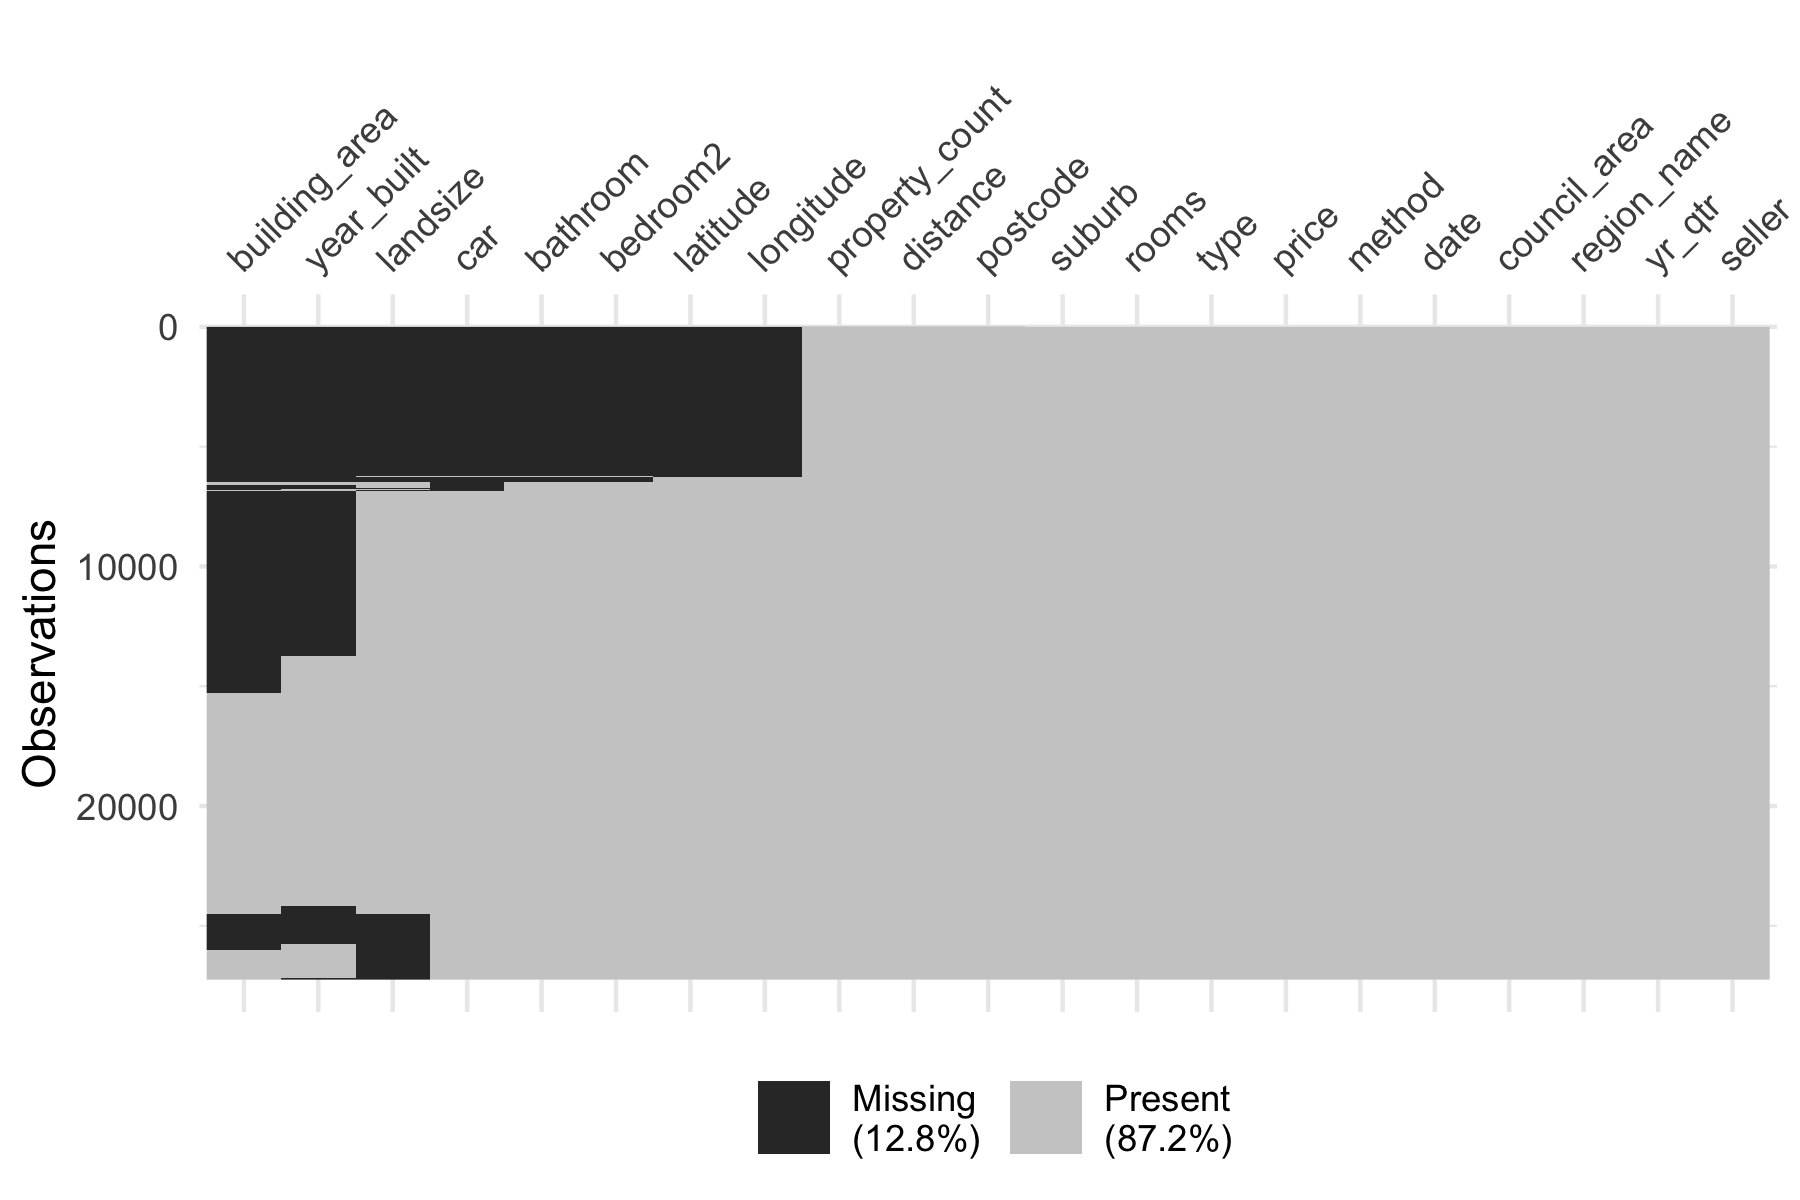
\includegraphics[width=0.85\linewidth]{figure/code-Rnwapplic-vis-miss-1} 

}

\caption[Heatmap of clustered missingness for housing data reveals structured missingness]{Heatmap of clustered missingness for housing data reveals structured missingness. Three groups of missingness are apparent. At the top: building area to longitude; the middle: building area and year built; the end: building area, year built, and landsize.}\label{fig:applic-vis-miss}
\end{figure}

\end{knitrout}
\begin{knitrout}
\definecolor{shadecolor}{rgb}{0.969, 0.969, 0.969}\color{fgcolor}\begin{kframe}
\begin{alltt}
\hlkwd{gg_miss_upset}\hlstd{(housing,}
              \hlkwc{nsets} \hlstd{=} \hlnum{8}\hlstd{,}
              \hlkwc{order.by} \hlstd{=} \hlstr{"freq"}\hlstd{)}
\end{alltt}
\end{kframe}\begin{figure}

{\centering \includegraphics[width=1\linewidth]{figure/code-Rnwhousing-upset-1} 

}

\caption[An upset plot of 8 sets of missingness in the housing data]{An upset plot of 8 sets of missingness in the housing data. Missingness for each variable is shown on the bottom left. Connected dots show co-occurences of missings in variables. Two missingness patterns are clear, year built and building area, and lattitude through to building area.}\label{fig:housing-upset}
\end{figure}

\end{knitrout}
\begin{knitrout}
\definecolor{shadecolor}{rgb}{0.969, 0.969, 0.969}\color{fgcolor}\begin{kframe}
\begin{alltt}
\hlstd{t1} \hlkwb{<-}  \hlkwd{miss_var_table}\hlstd{(housing)}
\hlstd{t2} \hlkwb{<-} \hlkwd{miss_case_table}\hlstd{(housing)}

\hlkwd{kable}\hlstd{(}\hlkwd{list}\hlstd{(t1, t2),}
             \hlkwc{caption} \hlstd{=} \hlstr{"Summary tables to help understand missingness patters. Output of \textbackslash{}\textbackslash{}code\{miss\textbackslash{}\textbackslash{}_var\textbackslash{}\textbackslash{}_table(housing)\} (left), tabulating missingness for variables, and output of \textbackslash{}\textbackslash{}code\{miss\textbackslash{}\textbackslash{}_case\textbackslash{}\textbackslash{}_table(housing)\}. There are 13 variables with 0-3 missings, 6 variables have 6000-10000 missings, 2 variables have 15000 – 17000 missings. About 30\textbackslash{}\textbackslash{}% of cases have no missings, 45\textbackslash{}\textbackslash{}% of cases have 1 - 6 missings, and about 23\textbackslash{}\textbackslash{}% of cases have 8 or more missings. There are different patterns of missingness in variables and cases, but they can be broken down into smaller groups."}\hlstd{,}
             \hlkwc{digits} \hlstd{=} \hlnum{1}\hlstd{)}
\end{alltt}
\end{kframe}\begin{table}
\caption{\label{tab:housing-miss-var-case-table}Summary tables to help understand missingness patters. Output of \code{miss\_var\_table(housing)} (left), tabulating missingness for variables, and output of \code{miss\_case\_table(housing)}. There are 13 variables with 0-3 missings, 6 variables have 6000-10000 missings, 2 variables have 15000 – 17000 missings. About 30\% of cases have no missings, 45\% of cases have 1 - 6 missings, and about 23\% of cases have 8 or more missings. There are different patterns of missingness in variables and cases, but they can be broken down into smaller groups.}

\centering
\begin{tabular}[t]{r|r|r}
\hline
n\_miss\_in\_var & n\_vars & pct\_vars\\
\hline
0 & 10 & 47.6\\
\hline
1 & 2 & 9.5\\
\hline
3 & 1 & 4.8\\
\hline
6254 & 2 & 9.5\\
\hline
6441 & 1 & 4.8\\
\hline
6447 & 1 & 4.8\\
\hline
6824 & 1 & 4.8\\
\hline
9265 & 1 & 4.8\\
\hline
15163 & 1 & 4.8\\
\hline
16591 & 1 & 4.8\\
\hline
\end{tabular}
\centering
\begin{tabular}[t]{r|r|r}
\hline
n\_miss\_in\_case & n\_cases & pct\_cases\\
\hline
0 & 8887 & 32.6\\
\hline
1 & 3237 & 11.9\\
\hline
2 & 7231 & 26.5\\
\hline
3 & 1370 & 5.0\\
\hline
4 & 79 & 0.3\\
\hline
5 & 8 & 0.0\\
\hline
6 & 203 & 0.7\\
\hline
8 & 6229 & 22.9\\
\hline
9 & 2 & 0.0\\
\hline
11 & 1 & 0.0\\
\hline
\end{tabular}
\end{table}

\begin{kframe}\begin{alltt}
             \hlcom{# booktabs = TRUE)}
  \hlcom{# kable_styling(latex_options = c("hold_position"))}
\end{alltt}
\end{kframe}
\end{knitrout}
\begin{knitrout}
\definecolor{shadecolor}{rgb}{0.969, 0.969, 0.969}\color{fgcolor}\begin{kframe}
\begin{alltt}
\hlstd{housing_cls} \hlkwb{<-} \hlkwd{add_miss_cluster}\hlstd{(housing,} \hlkwc{n_clusters} \hlstd{=} \hlnum{2}\hlstd{)}
\end{alltt}
\end{kframe}
\end{knitrout}
\begin{knitrout}
\definecolor{shadecolor}{rgb}{0.969, 0.969, 0.969}\color{fgcolor}\begin{kframe}
\begin{alltt}
\hlstd{miss_cls_pre_fit} \hlkwb{<-} \hlstd{housing_cls} \hlopt
  \hlkwd{mutate}\hlstd{(}\hlkwc{year} \hlstd{= lubridate}\hlopt{::}\hlkwd{year}\hlstd{(date),}
         \hlkwc{quarter} \hlstd{= lubridate}\hlopt{::}\hlkwd{quarter}\hlstd{(date))} \hlopt
  \hlkwd{mutate_at}\hlstd{(}\hlkwd{vars}\hlstd{(year, quarter),}
            \hlstd{as.factor)} \hlopt
  \hlkwd{select}\hlstd{(suburb,}
         \hlstd{council_area,}
         \hlstd{postcode,}
         \hlstd{method,}
         \hlstd{region_name,}
         \hlstd{rooms,}
         \hlstd{seller,}
         \hlstd{type,}
         \hlstd{year,}
         \hlstd{quarter,}
         \hlstd{price,}
         \hlstd{property_count,}
         \hlstd{distance,}
         \hlstd{latitude,}
         \hlstd{longitude,}
         \hlstd{miss_cluster)}
\hlstd{miss_cls_fit_rpart} \hlkwb{<-} \hlkwd{rpart}\hlstd{(}\hlkwd{factor}\hlstd{(miss_cluster)} \hlopt{~} \hlstd{.,}
                            \hlkwc{data} \hlstd{= miss_cls_pre_fit)}
\end{alltt}
\end{kframe}
\end{knitrout}
\begin{knitrout}
\definecolor{shadecolor}{rgb}{0.969, 0.969, 0.969}\color{fgcolor}\begin{kframe}
\begin{alltt}
\hlstd{rpart.plot}\hlopt{::}\hlkwd{prp}\hlstd{(miss_cls_fit_rpart,}
                \hlkwc{type} \hlstd{=} \hlnum{4}\hlstd{,}
                \hlkwc{extra} \hlstd{=} \hlnum{2}\hlstd{,}
                \hlkwc{fallen.leaves} \hlstd{=} \hlnum{TRUE}\hlstd{,}
                \hlkwc{prefix} \hlstd{=} \hlstr{"cluster = "}\hlstd{,}
                \hlkwc{suffix} \hlstd{=} \hlstr{" \textbackslash{}nObservations"}\hlstd{,}
                \hlkwc{box.col} \hlstd{=} \hlstr{"lightgrey"}\hlstd{,}
                \hlkwc{border.col} \hlstd{=} \hlstr{"grey"}\hlstd{,}
                \hlkwc{branch.col} \hlstd{=} \hlstr{"grey40"}\hlstd{)}
\end{alltt}
\end{kframe}\begin{figure}

{\centering \includegraphics[width=0.9\linewidth]{figure/code-Rnwrpart-plot-1} 

}

\caption[Decision tree output predicting missingness clusters]{Decision tree output predicting missingness clusters. Type of house, year quarter, and year were important for predicting missingness cluster. The cluster with the most missingness was for quarters 1 and 4, for 2017 and 2018. Type of house, year, and year quarter are important features related to missingness structure.}\label{fig:rpart-plot}
\end{figure}

\end{knitrout}
\begin{knitrout}
\definecolor{shadecolor}{rgb}{0.969, 0.969, 0.969}\color{fgcolor}\begin{kframe}
\begin{alltt}
\hlstd{data_in} \hlkwb{<-} \hlstd{housing_cls} \hlopt
  \hlkwd{mutate}\hlstd{(}\hlkwc{year} \hlstd{= lubridate}\hlopt{::}\hlkwd{year}\hlstd{(date),}
         \hlkwc{month} \hlstd{= lubridate}\hlopt{::}\hlkwd{month}\hlstd{(date),}
         \hlkwc{quarter} \hlstd{= lubridate}\hlopt{::}\hlkwd{quarter}\hlstd{(date))} \hlopt
  \hlkwd{mutate_at}\hlstd{(}\hlkwd{vars}\hlstd{(year, month, quarter),}
            \hlstd{as.factor)}

\hlstd{node_1} \hlkwb{<-} \hlstd{data_in} \hlopt
  \hlkwd{filter}\hlstd{(type} \hlopt{==} \hlstr{"h"}\hlstd{)}

\hlstd{node_2} \hlkwb{<-} \hlstd{data_in} \hlopt
  \hlkwd{filter}\hlstd{(type} \hlopt{!=} \hlstr{"h"}\hlstd{,}
         \hlstd{quarter} \hlopt{==} \hlnum{2} \hlopt{|} \hlstd{quarter} \hlopt{==} \hlnum{3}\hlstd{)}

\hlstd{node_3} \hlkwb{<-} \hlstd{data_in} \hlopt
  \hlkwd{filter}\hlstd{(type} \hlopt{!=} \hlstr{"h"}\hlstd{,}
         \hlstd{quarter} \hlopt{==} \hlnum{1} \hlopt{|} \hlstd{quarter} \hlopt{==} \hlnum{4}\hlstd{,}
         \hlstd{year} \hlopt{==} \hlnum{2016}\hlstd{)}

\hlstd{node_4} \hlkwb{<-} \hlstd{data_in} \hlopt
  \hlkwd{filter}\hlstd{(type} \hlopt{!=} \hlstr{"h"}\hlstd{,}
         \hlstd{quarter} \hlopt{==} \hlnum{1} \hlopt{|} \hlstd{quarter} \hlopt{==} \hlnum{4}\hlstd{,}
         \hlstd{year} \hlopt{==} \hlnum{2017} \hlopt{|} \hlstd{year} \hlopt{==} \hlnum{2018}\hlstd{)}
\end{alltt}
\end{kframe}
\end{knitrout}

\begin{knitrout}
\definecolor{shadecolor}{rgb}{0.969, 0.969, 0.969}\color{fgcolor}\begin{kframe}
\begin{alltt}
\hlkwd{set.seed}\hlstd{(}\hlnum{2022}\hlopt{-}\hlnum{12}\hlopt{-}\hlnum{1}\hlstd{)}
\hlstd{dat_house_lm} \hlkwb{<-} \hlstd{dat_house} \hlopt
  \hlkwd{nabular}\hlstd{()} \hlopt
  \hlkwd{as.data.frame}\hlstd{()} \hlopt
  \hlcom{# postcode}
  \hlkwd{impute_knn}\hlstd{(postcode} \hlopt{~} \hlstd{type} \hlopt{+} \hlstd{quarter} \hlopt{+} \hlstd{year} \hlopt{+} \hlstd{rooms} \hlopt{+} \hlstd{price} \hlopt{+} \hlstd{distance)} \hlopt
  \hlcom{# distance}
  \hlkwd{impute_lm}\hlstd{(distance} \hlopt{~} \hlstd{type} \hlopt{+} \hlstd{quarter} \hlopt{+} \hlstd{year} \hlopt{+} \hlstd{rooms} \hlopt{+} \hlstd{price)} \hlopt
  \hlcom{# property_count}
  \hlkwd{impute_lm}\hlstd{(property_count} \hlopt{~} \hlstd{type} \hlopt{+} \hlstd{quarter} \hlopt{+} \hlstd{year} \hlopt{+} \hlstd{rooms} \hlopt{+} \hlstd{price} \hlopt{+} \hlstd{distance)} \hlopt
  \hlcom{# longitude}
  \hlkwd{impute_lm}\hlstd{(longitude} \hlopt{~} \hlstd{type} \hlopt{+} \hlstd{quarter} \hlopt{+} \hlstd{year} \hlopt{+} \hlstd{rooms} \hlopt{+} \hlstd{price} \hlopt{+} \hlstd{distance)} \hlopt
  \hlcom{# latitude}
  \hlkwd{impute_lm}\hlstd{(latitude} \hlopt{~}  \hlstd{type} \hlopt{+} \hlstd{quarter} \hlopt{+} \hlstd{year} \hlopt{+} \hlstd{rooms} \hlopt{+} \hlstd{price} \hlopt{+} \hlstd{distance)} \hlopt
  \hlcom{# bedroom2}
  \hlkwd{impute_lm}\hlstd{(bedroom2} \hlopt{~}  \hlstd{type} \hlopt{+} \hlstd{quarter} \hlopt{+} \hlstd{year} \hlopt{+} \hlstd{rooms} \hlopt{+} \hlstd{price} \hlopt{+} \hlstd{distance)} \hlopt
  \hlcom{# bathroom}
  \hlkwd{impute_lm}\hlstd{(bathroom} \hlopt{~}  \hlstd{type} \hlopt{+} \hlstd{quarter} \hlopt{+} \hlstd{year} \hlopt{+} \hlstd{rooms} \hlopt{+} \hlstd{price} \hlopt{+} \hlstd{distance)} \hlopt
  \hlcom{# car}
  \hlkwd{impute_lm}\hlstd{(car} \hlopt{~} \hlstd{type} \hlopt{+} \hlstd{quarter} \hlopt{+} \hlstd{year} \hlopt{+} \hlstd{rooms} \hlopt{+} \hlstd{price} \hlopt{+} \hlstd{distance)} \hlopt
  \hlcom{# landsize}
  \hlkwd{impute_lm}\hlstd{(landsize} \hlopt{~}  \hlstd{type} \hlopt{+} \hlstd{quarter} \hlopt{+} \hlstd{year} \hlopt{+} \hlstd{rooms} \hlopt{+} \hlstd{price} \hlopt{+} \hlstd{distance)} \hlopt
  \hlkwd{add_label_shadow}\hlstd{()} \hlopt
  \hlcom{# recode integers back}
  \hlkwd{mutate_at}\hlstd{(}\hlkwd{vars}\hlstd{(bedroom2, bathroom, car), as.integer)}
\end{alltt}
\end{kframe}
\end{knitrout}
\begin{knitrout}
\definecolor{shadecolor}{rgb}{0.969, 0.969, 0.969}\color{fgcolor}\begin{kframe}
\begin{alltt}
\hlstd{dat_house_cc} \hlkwb{<-} \hlstd{dat_house} \hlopt \hlkwd{nabular}\hlstd{()} \hlopt \hlkwd{add_label_shadow}\hlstd{()} \hlopt \hlkwd{na.omit}\hlstd{()}

\hlstd{bound_models} \hlkwb{<-} \hlkwd{bind_rows}\hlstd{(}\hlkwc{lm} \hlstd{= dat_house_lm,}
                          \hlkwc{knn} \hlstd{= dat_house_knn,}
                          \hlkwc{cc} \hlstd{= dat_house_cc,}
                          \hlkwc{.id} \hlstd{=} \hlstr{"imp_model"}\hlstd{)} \hlopt
  \hlkwd{as_tibble}\hlstd{()}
\end{alltt}
\end{kframe}
\end{knitrout}
\begin{knitrout}
\definecolor{shadecolor}{rgb}{0.969, 0.969, 0.969}\color{fgcolor}\begin{kframe}
\begin{alltt}
\hlcom{## Now we want to look at the distribution of the values, so we need to do}
\hlcom{## some gathering}
\hlstd{bound_models_gather} \hlkwb{<-} \hlstd{bound_models} \hlopt
  \hlkwd{select}\hlstd{(}
         \hlstd{bedroom2,}
         \hlstd{bathroom,}
         \hlstd{car,}
         \hlstd{landsize,}
         \hlstd{any_missing,}
         \hlstd{imp_model)} \hlopt
  \hlkwd{gather}\hlstd{(}\hlkwc{key} \hlstd{=} \hlstr{"key"}\hlstd{,}
         \hlkwc{value} \hlstd{=} \hlstr{"value"}\hlstd{,}
         \hlopt{-}\hlstd{any_missing,}
         \hlopt{-}\hlstd{imp_model)}

\hlstd{p1} \hlkwb{<-} \hlstd{bound_models} \hlopt
  \hlkwd{ggplot}\hlstd{(}\hlkwd{aes}\hlstd{(}\hlkwc{x} \hlstd{= imp_model,}
             \hlkwc{y} \hlstd{= bedroom2))} \hlopt{+}
  \hlkwd{geom_boxplot}\hlstd{()}

\hlstd{p2} \hlkwb{<-} \hlstd{bound_models} \hlopt
  \hlkwd{ggplot}\hlstd{(}\hlkwd{aes}\hlstd{(}\hlkwc{x} \hlstd{= imp_model,}
             \hlkwc{y} \hlstd{= bathroom))} \hlopt{+}
  \hlkwd{geom_boxplot}\hlstd{()}

\hlstd{p3} \hlkwb{<-} \hlstd{bound_models} \hlopt
  \hlkwd{ggplot}\hlstd{(}\hlkwd{aes}\hlstd{(}\hlkwc{x} \hlstd{= imp_model,}
             \hlkwc{y} \hlstd{= car))} \hlopt{+}
  \hlkwd{geom_boxplot}\hlstd{()}

\hlstd{p4} \hlkwb{<-} \hlstd{bound_models} \hlopt
  \hlkwd{ggplot}\hlstd{(}\hlkwd{aes}\hlstd{(}\hlkwc{x} \hlstd{= imp_model,}
             \hlkwc{y} \hlstd{= landsize))} \hlopt{+}
  \hlkwd{geom_boxplot}\hlstd{()} \hlopt{+}
  \hlkwd{scale_y_log10}\hlstd{()}

\hlstd{cowplot}\hlopt{::}\hlkwd{plot_grid}\hlstd{(p1,}
          \hlstd{p2,}
          \hlstd{p3,}
          \hlstd{p4,}
          \hlkwc{nrow} \hlstd{=} \hlnum{1}\hlstd{,}
          \hlkwc{labels} \hlstd{=} \hlstr{"AUTO"}\hlstd{)}
\end{alltt}


{\ttfamily\noindent\color{warningcolor}{\#\# Warning in self\$trans\$transform(x): NaNs produced}}

{\ttfamily\noindent\color{warningcolor}{\#\# Warning: Transformation introduced infinite values in continuous y-axis}}

{\ttfamily\noindent\color{warningcolor}{\#\# Warning: Removed 5891 rows containing non-finite values (`stat\_boxplot()`).}}\end{kframe}\begin{figure}

{\centering \includegraphics[width=0.95\linewidth]{figure/code-Rnwimputed-by-model-1} 

}

\caption[Boxplots of complete case data, and data imputed with KNN or linear model for different variables]{Boxplots of complete case data, and data imputed with KNN or linear model for different variables. (A) number of bedrooms, (B) number of bathrooms, (C) number of carspots, and (D) landsize (on a log10 scale). KNN had similar results to complete case, and linear model had a lower median for cars and fewer extreme values for bedrooms.}\label{fig:imputed-by-model}
\end{figure}

\end{knitrout}
\begin{knitrout}
\definecolor{shadecolor}{rgb}{0.969, 0.969, 0.969}\color{fgcolor}\begin{kframe}
\begin{alltt}
\hlkwd{set.seed}\hlstd{(}\hlnum{2022}\hlopt{-}\hlnum{12}\hlopt{-}\hlnum{1}\hlstd{)}
\hlstd{dat_fit} \hlkwb{<-} \hlstd{dat_house} \hlopt
  \hlkwd{mutate_at}\hlstd{(}\hlkwd{vars}\hlstd{(car,}
                 \hlstd{bathroom,}
                 \hlstd{bedroom2,}
                 \hlstd{type,}
                 \hlstd{year,}
                 \hlstd{quarter,}
                 \hlstd{rooms),}
            \hlkwc{.funs} \hlstd{= as.factor)}

\hlstd{dat_fit_knn} \hlkwb{<-}  \hlstd{dat_house_knn} \hlopt
  \hlkwd{mutate_at}\hlstd{(}\hlkwd{vars}\hlstd{(car,}
                 \hlstd{bathroom,}
                 \hlstd{bedroom2,}
                 \hlstd{type,}
                 \hlstd{year,}
                 \hlstd{quarter,}
                 \hlstd{rooms),}
            \hlkwc{.funs} \hlstd{= as.factor)}

\hlstd{dat_fit_lm} \hlkwb{<-}  \hlstd{dat_house_lm} \hlopt
  \hlkwd{mutate_at}\hlstd{(}\hlkwd{vars}\hlstd{(car,}
                 \hlstd{bathroom,}
                 \hlstd{bedroom2,}
                 \hlstd{type,}
                 \hlstd{year,}
                 \hlstd{quarter,}
                 \hlstd{rooms),}
            \hlkwc{.funs} \hlstd{= as.factor)}

\hlstd{dat_house_cc} \hlkwb{<-} \hlkwd{na.omit}\hlstd{(dat_fit)}

\hlstd{fit_lm_dat_house_cc} \hlkwb{<-} \hlkwd{lm}\hlstd{(price} \hlopt{~} \hlstd{landsize} \hlopt{+}
                            \hlstd{car} \hlopt{+}
                            \hlstd{bathroom} \hlopt{+}
                            \hlstd{bedroom2} \hlopt{+}
                            \hlstd{type} \hlopt{+}
                            \hlstd{year} \hlopt{+}
                            \hlstd{quarter} \hlopt{+}
                            \hlstd{rooms} \hlopt{+}
                            \hlstd{distance,}
                          \hlstd{dat_house_cc)}

\hlstd{fit_lm_dat_house_knn} \hlkwb{<-} \hlkwd{lm}\hlstd{(price} \hlopt{~} \hlstd{landsize} \hlopt{+}
                            \hlstd{car} \hlopt{+}
                            \hlstd{bathroom} \hlopt{+}
                            \hlstd{bedroom2} \hlopt{+}
                            \hlstd{type} \hlopt{+}
                            \hlstd{year} \hlopt{+}
                            \hlstd{quarter} \hlopt{+}
                            \hlstd{rooms} \hlopt{+}
                            \hlstd{distance,}
                           \hlstd{dat_fit_knn)}

\hlstd{fit_lm_dat_house_lm} \hlkwb{<-} \hlkwd{lm}\hlstd{(price} \hlopt{~} \hlstd{landsize} \hlopt{+}
                            \hlstd{car} \hlopt{+}
                            \hlstd{bathroom} \hlopt{+}
                            \hlstd{bedroom2} \hlopt{+}
                            \hlstd{type} \hlopt{+}
                            \hlstd{year} \hlopt{+}
                            \hlstd{quarter} \hlopt{+}
                            \hlstd{rooms} \hlopt{+}
                            \hlstd{distance,}
                          \hlstd{dat_fit_lm)}
\end{alltt}
\end{kframe}
\end{knitrout}
\begin{knitrout}
\definecolor{shadecolor}{rgb}{0.969, 0.969, 0.969}\color{fgcolor}\begin{kframe}
\begin{alltt}
\hlstd{tidy_fit_cc} \hlkwb{<-} \hlstd{broom}\hlopt{::}\hlkwd{tidy}\hlstd{(fit_lm_dat_house_cc)}
\hlstd{tidy_fit_knn} \hlkwb{<-} \hlstd{broom}\hlopt{::}\hlkwd{tidy}\hlstd{(fit_lm_dat_house_knn)}
\hlstd{tidy_fit_lm} \hlkwb{<-} \hlstd{broom}\hlopt{::}\hlkwd{tidy}\hlstd{(fit_lm_dat_house_lm)}

\hlstd{tidy_fits} \hlkwb{<-} \hlkwd{bind_rows}\hlstd{(}\hlkwc{cc} \hlstd{= tidy_fit_cc,}
                       \hlkwc{knn} \hlstd{= tidy_fit_knn,}
                       \hlkwc{lm} \hlstd{= tidy_fit_lm,}
                       \hlkwc{.id} \hlstd{=} \hlstr{"model"}\hlstd{)}

\hlstd{tidy_fits_data} \hlkwb{<-}  \hlstd{tidy_fits} \hlopt
  \hlkwd{filter}\hlstd{(term} \hlopt{!=} \hlstr{"(Intercept)"}\hlstd{)} \hlopt
  \hlkwd{filter}\hlstd{(}\hlkwd{grepl}\hlstd{(}\hlstr{"rooms"}\hlstd{, term))} \hlopt
  \hlkwd{select}\hlstd{(model, term, estimate)} \hlopt
  \hlkwd{spread}\hlstd{(}\hlkwc{key} \hlstd{= model,}
         \hlkwc{value} \hlstd{= estimate)}

\hlstd{tidy_fits} \hlopt
  \hlkwd{filter}\hlstd{(term} \hlopt{!=} \hlstr{"(Intercept)"}\hlstd{)} \hlopt
  \hlkwd{filter}\hlstd{(}\hlkwd{grepl}\hlstd{(}\hlstr{"rooms"}\hlstd{, term))} \hlopt
  \hlkwd{select}\hlstd{(model, term, estimate)} \hlopt
  \hlkwd{ggplot}\hlstd{(}\hlkwd{aes}\hlstd{(}\hlkwc{x} \hlstd{= estimate,}
             \hlkwc{y} \hlstd{= term,}
             \hlkwc{colour} \hlstd{= model))} \hlopt{+}
  \hlkwd{geom_point}\hlstd{()} \hlopt{+}
  \hlkwd{theme_minimal}\hlstd{()} \hlopt{+}
  \hlkwd{labs}\hlstd{(}\hlkwc{x} \hlstd{=} \hlstr{"Estimate"}\hlstd{,}
       \hlkwc{y} \hlstd{=} \hlstr{"Term"}\hlstd{)} \hlopt{+}
  \hlkwd{guides}\hlstd{(}\hlkwc{colour} \hlstd{=} \hlkwd{guide_legend}\hlstd{(}\hlkwc{title} \hlstd{=} \hlstr{"Model"}\hlstd{))}
\end{alltt}
\end{kframe}\begin{figure}

{\centering \includegraphics[width=1\linewidth]{figure/code-Rnwtidy-coefs-1} 

}

\caption[The coefficient estimate for the number of rooms varies according to the imputed dataset]{The coefficient estimate for the number of rooms varies according to the imputed dataset. Complete case dataset produced lower coefficients, compared to imputed datasets.}\label{fig:tidy-coefs}
\end{figure}

\end{knitrout}
\begin{knitrout}
\definecolor{shadecolor}{rgb}{0.969, 0.969, 0.969}\color{fgcolor}\begin{kframe}
\begin{alltt}
\hlstd{aug_fit_cc} \hlkwb{<-}  \hlstd{broom}\hlopt{::}\hlkwd{augment}\hlstd{(fit_lm_dat_house_cc)} \hlopt \hlkwd{as_tibble}\hlstd{()}
\hlstd{aug_fit_knn} \hlkwb{<-} \hlstd{broom}\hlopt{::}\hlkwd{augment}\hlstd{(fit_lm_dat_house_knn)} \hlopt \hlkwd{as_tibble}\hlstd{()}
\hlstd{aug_fit_lm} \hlkwb{<-}  \hlstd{broom}\hlopt{::}\hlkwd{augment}\hlstd{(fit_lm_dat_house_lm)}\hlopt \hlkwd{as_tibble}\hlstd{()}

\hlstd{aug_fits} \hlkwb{<-} \hlkwd{bind_rows}\hlstd{(}\hlkwc{cc} \hlstd{=  aug_fit_cc,}
                      \hlkwc{knn} \hlstd{= aug_fit_knn,}
                      \hlkwc{lm} \hlstd{=  aug_fit_lm,}
                      \hlkwc{.id} \hlstd{=} \hlstr{"model"}\hlstd{)}

\hlkwd{ggplot}\hlstd{(aug_fits,} \hlkwd{aes}\hlstd{(}\hlkwc{x} \hlstd{= .fitted,}
                     \hlkwc{y} \hlstd{= .resid))} \hlopt{+}
  \hlkwd{stat_density_2d}\hlstd{(}
    \hlkwc{geom} \hlstd{=} \hlstr{"polygon"}\hlstd{,}
    \hlkwc{contour} \hlstd{=} \hlnum{TRUE}\hlstd{,}
    \hlkwd{aes}\hlstd{(}\hlkwc{fill} \hlstd{=} \hlkwd{after_stat}\hlstd{(level)),}
    \hlkwc{bins} \hlstd{=} \hlnum{7}
  \hlstd{)} \hlopt{+}
  \hlkwd{facet_wrap}\hlstd{(}\hlkwd{vars}\hlstd{(model))} \hlopt{+}
  \hlkwd{scale_fill_viridis_c}\hlstd{()} \hlopt{+}
  \hlkwd{theme_bw}\hlstd{()} \hlopt{+}
  \hlkwd{scale_x_continuous}\hlstd{(}\hlkwc{n.breaks} \hlstd{=} \hlnum{4}\hlstd{)} \hlopt{+}
  \hlkwd{scale_y_continuous}\hlstd{(}\hlkwc{n.breaks} \hlstd{=} \hlnum{4}\hlstd{)} \hlopt{+}
  \hlkwd{theme}\hlstd{(}\hlkwc{legend.position} \hlstd{=} \hlstr{"none"}\hlstd{,}
        \hlkwc{aspect.ratio} \hlstd{=} \hlnum{1}\hlstd{)}
\end{alltt}
\end{kframe}\begin{figure}

{\centering \includegraphics[width=1\linewidth]{figure/code-Rnwpartial-resid-1} 

}

\caption[Partial residual plot for each data set, complete cases (cc), and imputed with KNN (knn) or linear model (lm)]{Partial residual plot for each data set, complete cases (cc), and imputed with KNN (knn) or linear model (lm). These are plotted as two dimensional filled density plots with 7 bins estimated. The bins are colored according to concentration of points in that area - brighter colors indicated higher concentration. Compared to complete cases, imputed data has more points clustered closer to 0 for residuals, and and around 6 fitted values.}\label{fig:partial-resid}
\end{figure}

\end{knitrout}

The R session information (including the OS info, R version and all
packages used):

\begin{knitrout}
\definecolor{shadecolor}{rgb}{0.969, 0.969, 0.969}\color{fgcolor}\begin{kframe}
\begin{alltt}
\hlkwd{sessionInfo}\hlstd{()}
\end{alltt}
\begin{verbatim}
## R version 4.2.1 (2022-06-23)
## Platform: aarch64-apple-darwin20 (64-bit)
## Running under: macOS Monterey 12.3.1
## 
## Matrix products: default
## LAPACK: /Library/Frameworks/R.framework/Versions/4.2-arm64/Resources/lib/libRlapack.dylib
## 
## locale:
## [1] en_US.UTF-8/en_US.UTF-8/en_US.UTF-8/C/en_US.UTF-8/en_US.UTF-8
## 
## attached base packages:
## [1] stats     graphics  grDevices utils     datasets  methods   base     
## 
## other attached packages:
##  [1] cowplot_1.1.1     knitr_1.41        janitor_2.1.0     targets_0.14.0   
##  [5] withr_2.5.0       patchwork_1.1.2   visdat_0.5.3      rpart_4.1.19     
##  [9] magick_2.7.3      lubridate_1.9.0   timechange_0.1.1  naniar_0.6.1     
## [13] simputation_0.2.8 scales_1.2.1      png_0.1-7         ggthemes_4.2.4   
## [17] gridExtra_2.3     forcats_0.5.2     stringr_1.4.1     dplyr_1.0.10     
## [21] purrr_0.3.5       readr_2.1.3       tidyr_1.2.1       tibble_3.1.8     
## [25] ggplot2_3.4.0     tidyverse_1.3.2   gert_1.9.1        clipr_0.8.0      
## [29] pak_0.3.1         fs_1.5.2          testthat_3.1.5    devtools_2.4.5   
## [33] usethis_2.1.6    
## 
## loaded via a namespace (and not attached):
##  [1] googledrive_2.0.0   colorspace_2.0-3    ellipsis_0.3.2      snakecase_0.11.0   
##  [5] rstudioapi_0.14     farver_2.1.1        remotes_2.4.2       bit64_4.0.5        
##  [9] fansi_1.0.3         xml2_1.3.3          codetools_0.2-18    cachem_1.0.6       
## [13] pkgload_1.3.2       jsonlite_1.8.3      broom_1.0.1         dbplyr_2.2.1       
## [17] shiny_1.7.3         compiler_4.2.1      httr_1.4.4          backports_1.4.1    
## [21] assertthat_0.2.1    fastmap_1.1.0       gargle_1.2.1        cli_3.4.1          
## [25] later_1.3.0         htmltools_0.5.3     prettyunits_1.1.1   tools_4.2.1        
## [29] igraph_1.3.5        gtable_0.3.1        glue_1.6.2          Rcpp_1.0.9         
## [33] cellranger_1.1.0    vctrs_0.5.1         xfun_0.35           gower_1.0.0        
## [37] ps_1.7.2            brio_1.1.3          rvest_1.0.3         mime_0.12          
## [41] miniUI_0.1.1.1      lifecycle_1.0.3     sys_3.4.1           googlesheets4_1.0.1
## [45] MASS_7.3-58.1       vroom_1.6.0         hms_1.1.2           promises_1.2.0.1   
## [49] credentials_1.3.2   parallel_4.2.1      RColorBrewer_1.1-3  rpart.plot_3.1.1   
## [53] yaml_2.3.6          curl_4.3.3          memoise_2.0.1       UpSetR_1.4.0       
## [57] stringi_1.7.8       highr_0.9           pkgbuild_1.4.0      rlang_1.0.6        
## [61] pkgconfig_2.0.3     evaluate_0.18       labeling_0.4.2      htmlwidgets_1.5.4  
## [65] bit_4.0.5           processx_3.8.0      tidyselect_1.2.0    plyr_1.8.8         
## [69] magrittr_2.0.3      R6_2.5.1            generics_0.1.3      profvis_0.3.7      
## [73] base64url_1.4       DBI_1.1.3           pillar_1.8.1        haven_2.5.1        
## [77] modelr_0.1.10       crayon_1.5.2        utf8_1.2.2          tzdb_0.3.0         
## [81] urlchecker_1.0.1    isoband_0.2.6       grid_4.2.1          readxl_1.4.1       
## [85] data.table_1.14.6   callr_3.7.3         reprex_2.0.2        digest_0.6.30      
## [89] xtable_1.8-4        httpuv_1.6.6        openssl_2.0.4       munsell_0.5.0      
## [93] viridisLite_0.4.1   sessioninfo_1.2.2   askpass_1.1
\end{verbatim}
\begin{alltt}
\hlkwd{Sys.time}\hlstd{()}
\end{alltt}
\begin{verbatim}
## [1] "2022-12-02 12:28:29 AWST"
\end{verbatim}
\end{kframe}
\end{knitrout}


\end{document}
